\begingroup
\centering
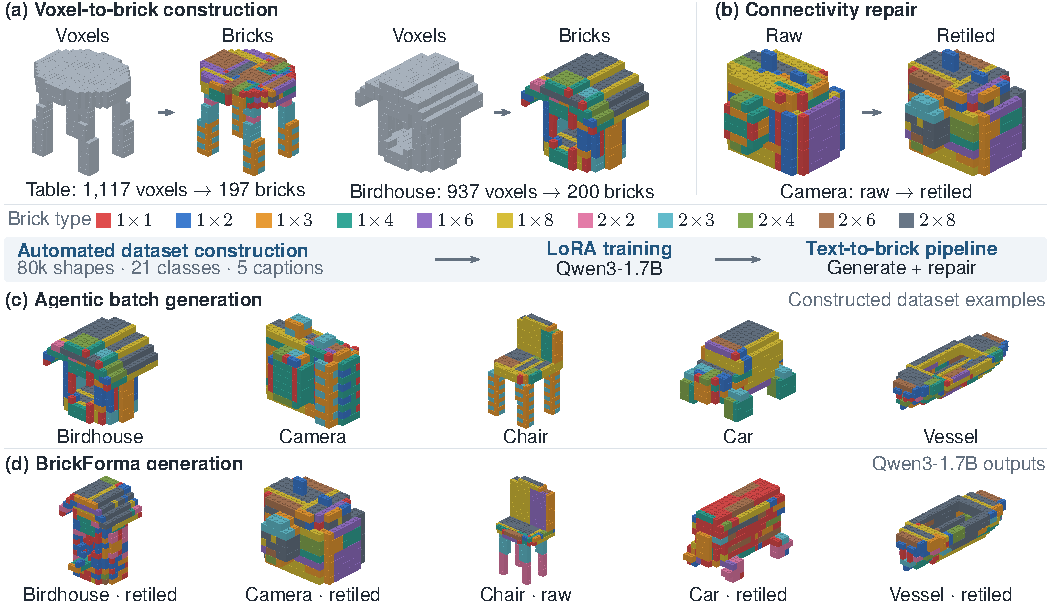
\includegraphics[width=\textwidth]{figure1.pdf}
\captionof{figure}{BrickForma overview. (a) Source voxels are converted into rectangular bricks. (b) Raw predictions are retiled to repair connectivity. (c) Brick layouts constructed from programmatically generated voxels. (d) Outputs of the fine-tuned Qwen3-1.7B pipeline. Colors encode brick type independent of orientation; they are visualization labels, not predicted appearance. Voxels are shown in gray.}
\label{fig:teaser}
\par\endgroup

